\section{Machine Learning}

Supervised learning, i.e.\ have labelled data.

Binary classification tasks: Every training example has a label indicating the class membership.

In HEP, the positive class is typically referred to as \emph{signal} while the
negative class is referred to as \emph{background}.



\subsection{Boosted Decision Trees}

Boosted decision trees (BDT) are a classification algorithm consisting on an
ensemble of \emph{decision tree classifiers} that are combined to yield a more
powerful classifier. This ensemble of decision trees is created using a
meta-algorithm referred to as \emph{boosting}






Boosted decision trees


ensemble of decision tree classifier

creat





A decision tree is a classification algorithm that partitions

into disjoint

\begin{figure}[htbp]
  \centering

  \begin{subfigure}{0.46\textwidth}
    \centering
    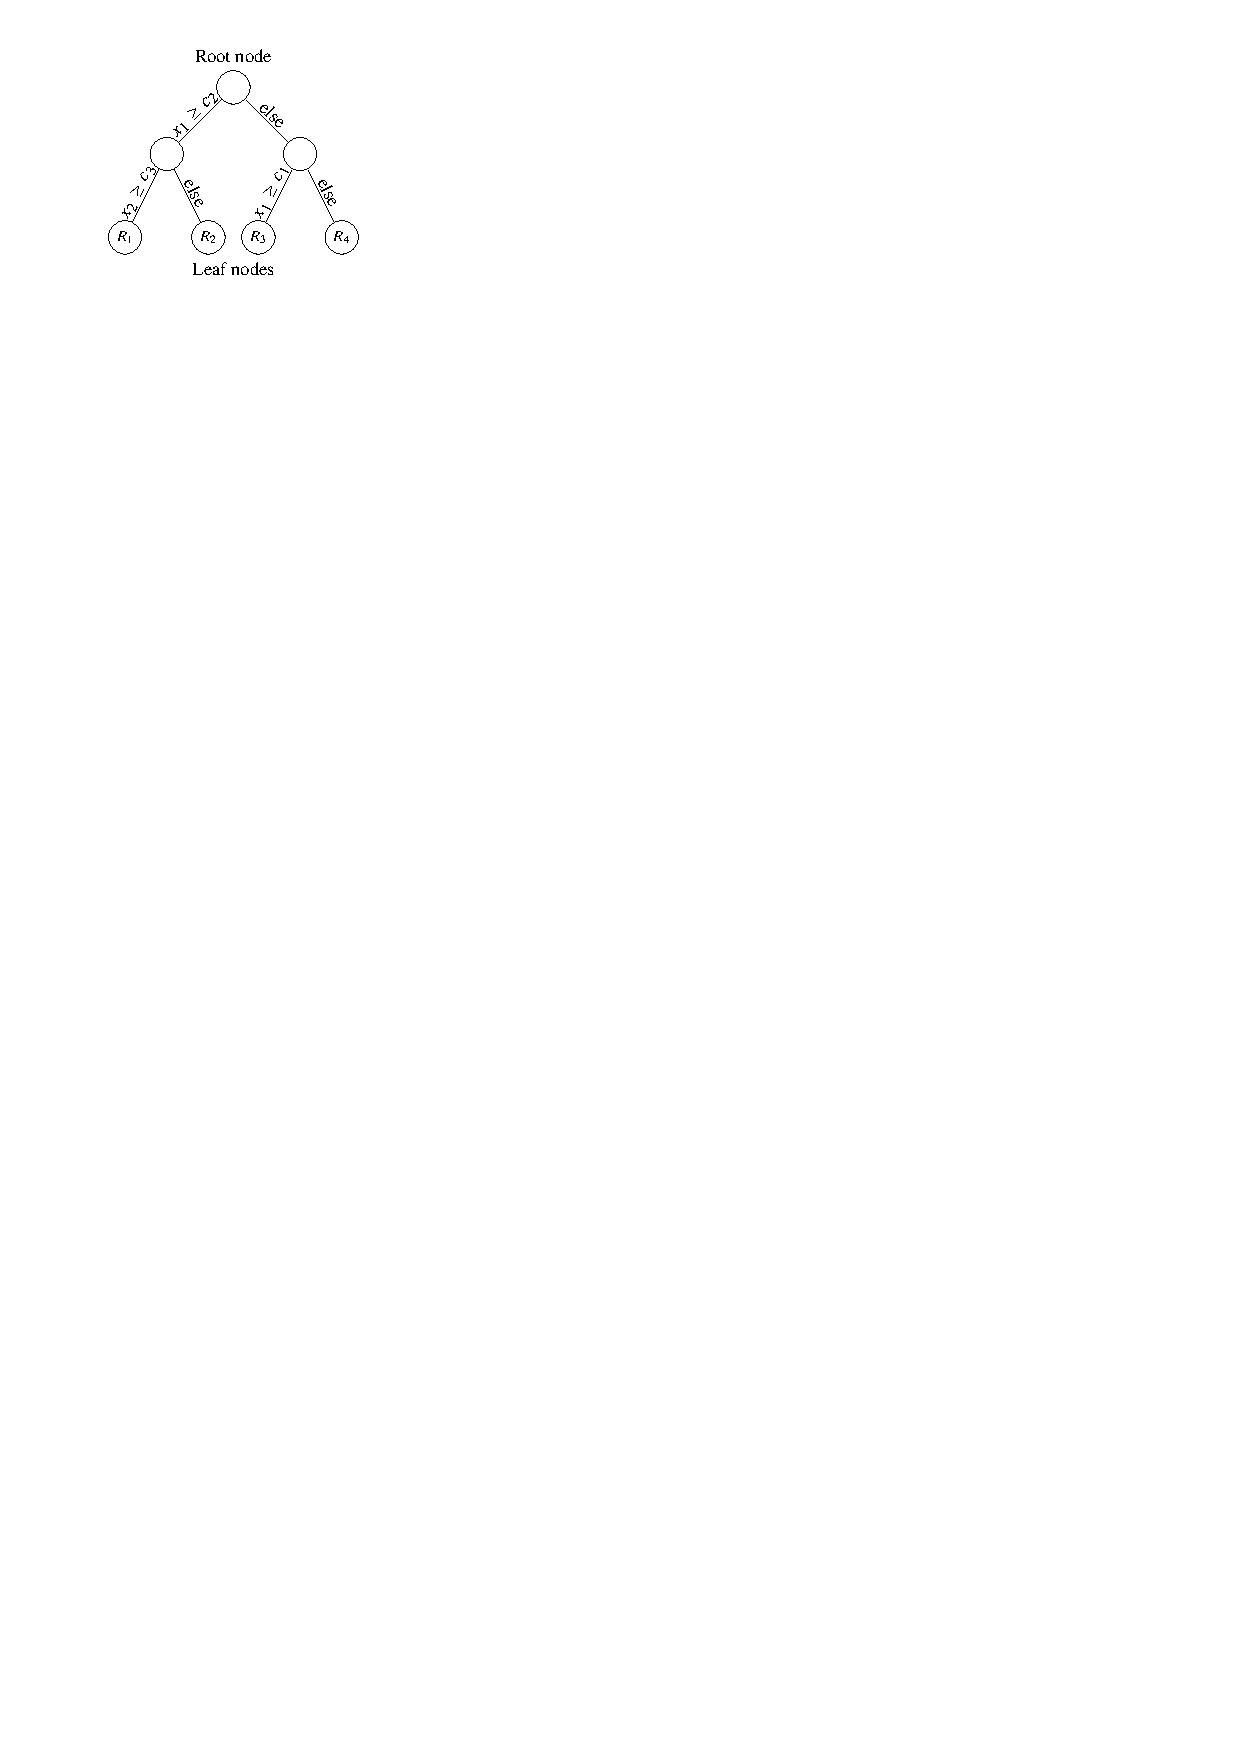
\includegraphics[scale=1.05]{ml/decision_tree}
    \caption{}
  \end{subfigure}\hfill%
  \begin{subfigure}{0.46\textwidth}
    \centering
    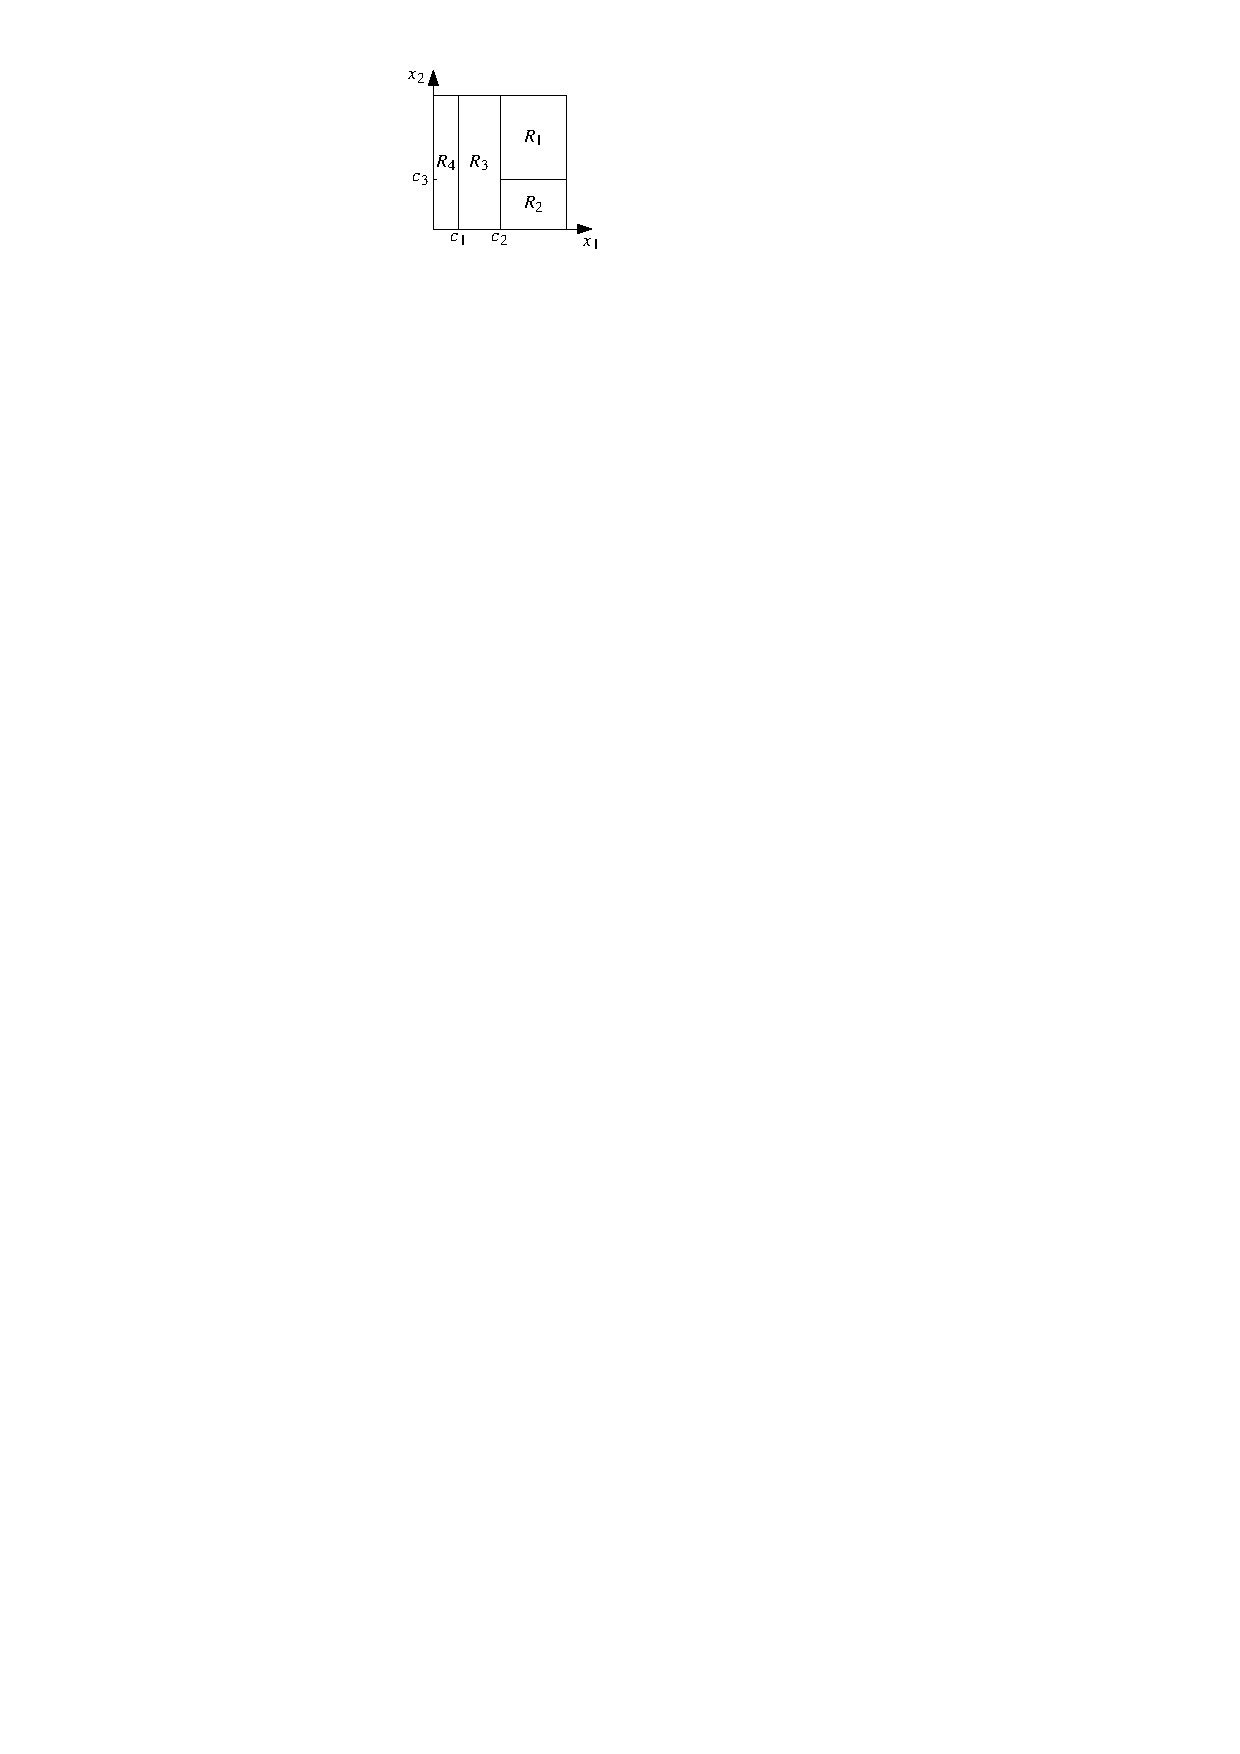
\includegraphics[scale=1.05]{ml/decision_tree_partitioning}
    \caption{}
  \end{subfigure}\hfill%

  \caption{abc. The figure is adapted from Ref.~\cite{hastie09}.}
  \label{fig:decision_tree}
\end{figure}





\subsection{Neural Networks}

\subsubsection{Recurrent Neural Networks}%
\label{sec:rnn}


%%% Local Variables:
%%% mode: latex
%%% TeX-master: "../../phd_thesis"
%%% End:
